\documentclass{book}
\usepackage{listings}
\usepackage{hyperref}
\usepackage{verbatim}
\usepackage{amsmath}
\usepackage[backend=bibtex, sorting=none, style=numeric-comp, defernumbers]{biblatex}
\usepackage{graphicx}

\addbibresource{\jobname.bib}

\begin{document}

\title{Chapter 2 - Supervised Learning }
\author {Joydeep Bhattacharjee}

\maketitle

\section{What is machine learning}
Machine learning is the science of getting computers to act without being specifically programmed. This is done by implementing special algorithms that have the ability to detect patterns in data. From a developer point of view this means creating a system, which has access to relevant data, is able to feed the data to machine learning algorithms and is able to take the output and redirect it to downstream processes and tasks.

\paragraph{Supervised learning}%
Supervised learning happens when you pass both the input and the desired outputs to the system and you want the resulting machine learning model to capture the relationship. Supervised learning are again divided into two subsections based on the type of the labels.

Supervised tasks when the target variable is continuous are termed as regression problems. For example the price of a product can be any value. We should probably go for regression techniques when the prediction needs to be made on something that requires the prediction of a quantity of some sort. Quality of a regression model is generally measured using some form of error measures, that is the difference between the target values and the predicted values.

Classifications problems are different from regression problems in that the labels are discrete and finite. For example, we can categorize an email message as spam or ham. So a problem is a classification problem when we are interested in the resulting bucket that a particular set of feature readings will fall into. Quality of a classification model is generally measured using an accuracy measure which is essentially the count of the number of times the model has been right.
\label{par:supervised_learning}

\paragraph{Unsupervised learning}%
In unsupervised algorithms the labels or the target classes are not given. So the goal of unsupervised learning is to attempt to find natural partitions of patterns.

The best time for unsupervised learning is when the data on desired outcomes is not known, such as creating a new class of products that the business has never sold before.
\label{par:unsupervised_learning}

\paragraph{Reinforcement learning}%
In reinforcement learning, specifically crafted agents are released in an environment, in which they learn to take actions based on some notion of rewards and punishments. Reinforcement learning has been applied to robotic movements and different classes of games with some success.
\label{par:reinforcement_learning}

In this chapter we will be taking a look at creating models for different machine learning algorithms using Rust. We will first read a data set from a csv file. This is a common data set and will be representative of the types of data in the real world. Then we will look at the logic of popular algorithms, why they work and how to implement them using some Rust ML packages such as \lstinline{rusty_machine}. Each different types of models will also include and understanding of how to evaluate those models in Rust.

By the end of this chapter you should have a fair understanding of how to create common ML models and implement them in Rust.

\label{sec:whatismachinelearning}

\section{Dataset specific code}%
Before going into regression algorithms and the associated code lets build the surrounding boilerplate code. Look at the $rusty\_machine\_regression$ package for the accompanying code in this.

For showing usage of regression we will be using the boston housing dataset\footnote{\href{https://www.cs.toronto.edu/~delve/data/boston/bostonDetail.html}{Housing dataset source}}. The dataset has 14 features and has 506 cases. Below is a description of the dataset.

\begin{itemize}
	\item CRIM - per capita crime rate by town
	\item ZN - proportion of residential land zoned for lots over 25,000 sq.ft.
	\item INDUS - proportion of non-retail business acres per town.
	\item CHAS - Charles River dummy variable (1 if tract bounds river; 0 otherwise)
	\item NOX - nitric oxides concentration (parts per 10 million)
	\item RM - average number of rooms per dwelling
	\item AGE - proportion of owner-occupied units built prior to 1940
	\item DIS - weighted distances to five Boston employment centres
	\item RAD - index of accessibility to radial highways
	\item TAX - full-value property-tax rate per \$10,000
	\item PTRATIO - pupil-teacher ratio by town
	\item B - 1000(Bk - 0.63)\^2 where Bk is the proportion of blacks by town
	\item LSTAT - \% lower status of the population
	\item MEDV - Median value of owner-occupied homes in \$1000's.
\end{itemize}

The data is kept in a file "data/housing.csv". A quick look at the csv suggests that it is a fixed width files with no headers.

\begin{lstlisting}[language=bash,caption={housing data}]
$ head -n1 data/housing.csv \
   | grep -Eo '[0-9]*[.]?[0-9]*' \
   | wc -l
14
$ head -n2 data/housing.csv
 0.00632  18.00   2.310  0  0.5380  6.5750  65.20  4.0900   1  296.0  15.30 396.90   4.98  24.00
 0.02731   0.00   7.070  0  0.4690  6.4210  78.90  4.9671   2  242.0  17.80 396.90   9.14  21.60
\end{lstlisting}

To parse through the files we will need these dependencies in our \lstinline{Cargo.toml} file.

\begin{lstlisting}[caption={Cargo.toml}]
[dependencies]
serde = "1"
serde_derive = "1"
rand = "0.6.5"
csv = "1.0.7"
\end{lstlisting}

For your applications go to the \lstinline{crates.io} page and use the latest version. For your specific page you can see that there s a search bar where you can put your search terms. In figure1, the \lstinline{csv} page is shown.

\begin{figure}[htpb]
	\centering
	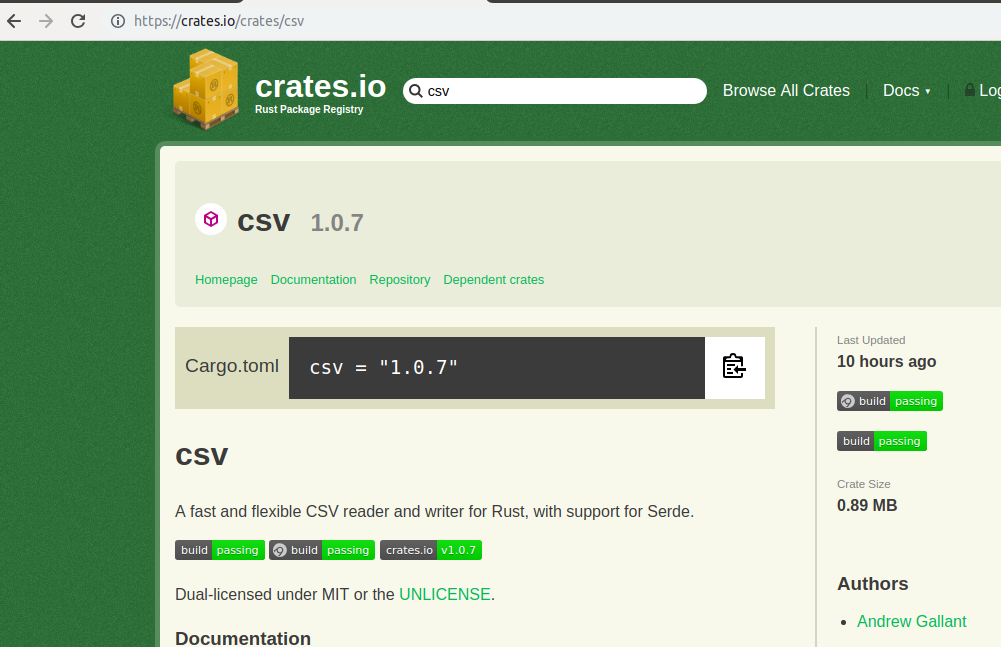
\includegraphics[width=0.8\linewidth]{cratesiopage.png}
	\caption{Crates page}
	\label{fig:crates page}
\end{figure}

If you scroll below you will get the accompanying documentation as well.

\paragraph{}%
And we will need to import the required modules in the module. Most of the code in this book has been written in Rust 2018 and hence we will not need explicit \lstinline{extern} crate statements for all the dependencies.
\label{par:import_required_modules}

\begin{lstlisting}[caption={regression}]
extern crate serde;
#[macro_use]
extern crate serde_derive;
use std::io::prelude::*;
use std::io::BufReader;
use std::path::Path;
use std::fs::File;
use std::vec::Vec;
use std::error::Error;
use rand::thread_rng;
use rand::seq::SliceRandom;
\end{lstlisting}

\paragraph{}%
To parse the file and match with appropriate records we create a \lstinline{struct} with each value to be a \lstinline{float64}\footnote{This does not mean that they cannot be used in 32-bit machines. Floats have nothing to do with the bitness of the machine.}. We will need to initialise them as \lstinline{float64} due to the Rust machine learning library to we will use that we will introduce later in this section.
\label{par:}

\begin{lstlisting}[caption={chapter2\\/ml\\-utils\\/src\\/datasets\\.rs}]
struct BostonHousing {
  crim: f64, cazn: f64, indus: f64, chas: f64, nox: f64,
  rm: f64, age: f64, dis: f64, rad: f64, tax: f64,
  ptratio: f64, black: f64, lstat: f64, medv: f64,
}
\end{lstlisting}

\paragraph{}%
One way to convert the file into records is to read the file line by line and build the \lstinline{BostonHousing} record. This should enable us to implement methods that separate out the predictors and the responses or target variables. In this case we consider the median value of the house (the price of the house) as the target and we will try to predict the price of the house based on the predictors available.
\label{par:}

\paragraph{}%
Below is the code to implement the building of a \lstinline{BostonHousing} record and methods to build the feature vector and targets.
\label{par:}

\begin{lstlisting}[caption={chapter2\\/ml\\-utils\\/src\\/datasets\\.rs}]
impl BostonHousing {
  fn new(v: Vec<&str>) -> BostonHousing {
    let n: Vec<f64> = v.iter().map(
      |s| s.parse().unwrap()).collect();
  BostonHousing { crim: n[0], zn: n[1],
    indus: n[2], chas: n[3], nox: n[4],
    rm: n[5], age: n[6], dis: n[7],
    rad: n[8], tax: n[9], ptratio: n[10],
    black: n[11], lstat: n[12], medv: n[13] }
  }

  fn into_feature_vector(&self) -> Vec<f64> {
    vec![self.crim, self.zn, self.indus, self.chas, self.nox,
      self.rm, self.age, self.dis, self.rad,
      self.tax, self.ptratio, self.black, self.lstat]
  }

  fn into_targets(&self) -> f64 {
    self.medv
  }
}
\end{lstlisting}

\paragraph{}%
Now that we can proceed and start reading the file line by line using \lstinline{get_boston_records_from_file}. Each line will be passed to the \lstinline{get_boston_record} function which splits the string to a vector of strings to be parsed appropriately by \lstinline{BostonRecord}. We assign this to a mutable variable data to be used later.
\label{par:}

\begin{lstlisting}[caption={chapter2\\/ml\\-utils\\/src\\/datasets\\.rs}]
fn get_boston_record(s: String) -> BostonHousing {
  let v: Vec<&str> = s.split_whitespace().collect();
  let b: BostonHousing = BostonHousing::new(v);
  b
}

fn get_boston_records_from_file(
    fl: impl AsRef<Path>) -> Vec<BostonHousing> {
  let file = File::open(fl).expect("no such file");
  let buf = BufReader::new(file);
  buf.lines().enumerate()
    .map(|(n, l)| l.expect(
       &format!("Could not parse line no {}", n)))
    .map(|r| get_boston_record(r))
    .collect()
}
\end{lstlisting}

We should now be able to call the function in our code.

\begin{lstlisting}[caption={chapter2\\/rustlymachine\_regression\\/src\\/lin\_reg\\.rs}]
use ml_utils::datasets::get_boston_records_from_file;

let fl = "data/housing.csv";
let mut data = get_boston_records_from_file(&fl);
\end{lstlisting}

\paragraph{}%
In machine learning tasks it is a good practice to shuffle the incoming dataset. Shuffling data serves the purpose of reducing variance and making sure that models remain general and overfit less. Shuffling helps in making sure that the train\\/test\\/validation samples of the dataset are representative of the overall distribution of the data.
\label{par:}

\paragraph{}%
Below we shuffle the data, split them into 80\% train and 20\% test and convert them into \lstinline{f64} vectors.
\label{par:}

\begin{lstlisting}[caption={chapter2\\/rustlymachine\_regression\\/src\\/lin\_reg\\.rs}]
data.shuffle(&mut thread_rng());

// separate out to train and test datasets.
let test_size: f64 = 0.2;
let test_size: f64 = data.len() as f64 * test_size;
let test_size = test_size.round() as usize;
let (test_data, train_data) = data.split_at(test_size);
let train_size = train_data.len();
let test_size = test_data.len();

// differentiate the predictors and the targets.
let boston_x_train: Vec<f64> = train_data.iter()
  .flat_map(|r| r.into_feature_vector())
  .collect();
let boston_y_train: Vec<f64> = train_data.iter()
  .map(|r| r.into_targets()).collect();
let boston_x_test: Vec<f64> = test_data.iter()
  .flat_map(|r| r.into_feature_vector()).collect();
let boston_y_test: Vec<f64> = test_data.iter()
  .map(|r| r.into_targets()).collect();
\end{lstlisting}

All of the above code has been kept in the \lstinline{datasets} module of the \lstinline{ml-utils} package.

\label{sub:dataset_specific_code}

\section{Rusty Machine Library}%

\paragraph{}%
Rusty machine is a general purpose machine learning library written entirely in Rust. The main aims of rusty-machine are ease of use and speed without having to depend on a huge number of external libraries. The consistency in the api is achieved using Rust’s trait system. It currently uses \lstinline{rulinalg} for its linear algebra backend. In this book one of the core libraries that we will focus on to achieve our machine learning needs is by using this library.
\label{par:}

\paragraph{}%
To use the rusty-machine library we will need to convert the data vectors into \lstinline{rulianalg} supported Matrices. Convert the above vectors like below.
\label{par:}

\begin{lstlisting}[caption={chapter2\\/rustlymachine\_regression\\/src\\/lin\_reg\\.rs}]
use rusty_machine;
use rusty_machine::linalg::Matrix;
use rusty_machine::linalg::Vector;

let boston_x_train = Matrix::new(train_size, 13, boston_x_train);
let boston_y_train = Vector::new(boston_y_train);
let boston_x_test = Matrix::new(test_size, 13, boston_x_test);
let boston_y_test = Matrix::new(test_size, 1, boston_y_test);
\end{lstlisting}

\paragraph{}%
In rusty-machine the two key methods that are implemented throughout is the \lstinline{train} and \lstinline{predict} methods.
\label{par:}

\label{sub:rusty_machine_library}

\section{Linear Regression}%

\paragraph{}%
Ordinary Least Squares linear regression is the method where a linear model with coefficients $w = (w1, w2, \dots, wp)$ to minimise the residual sum of squares between the observed responses in the dataset, and the responses predicted by the linear approximation. Mathematically it solves the problem of the form:
\label{par:}

\begin{equation}
	\underset{\omega}{\min} = || X\omega - y ||^2
\end{equation}

\paragraph{Rusty Machine}%
To optimise the model one of the methods is Gradient Descent. Train a linear regression model using the below code.

\begin{lstlisting}[caption={chapter2\\/rustlymachine\_regression\\/src\\/lin\_reg\\.rs}]
let mut lin_model = LinRegressor::default();
lin_model.train(&boston_x_train, &boston_y_train)?;
\end{lstlisting}

Creating a linear regression model similar to above is kept in the module \lstinline{chapter2/rustlymachine_regression/src/lin_reg.rs} module.
\label{par:}
\paragraph{Tensorflow}%
An interesting implementation of regression can be done using the closed form solution of the regression equation using tensorflow. Before going into the implementation using tensorflow I would suggest taking a look at the appendix for a creation of nodes and running a graph in tensorflow.

Tensorflow is designed in such a way that to implement computations we essentially need to create graphs. A tensorflow program is essentially divided into two parts. In one part we create the computational graph and then we write the code that runs the graph in a session. To solve linear regression using the normal equation where we solve for theta ($\hat{\theta} = (X^T \cdot X)^{-1}\cdot X^T \cdot y$) where $\hat{\theta}$ are the weights.

To create the computational graph we will first load the vectors to the tensors with the appropriate dimensions.

\begin{lstlisting}[caption={chapter\\/rust\_and\_tf\\/src\\/linear\_regression\\.rs}]
let dim = (boston_y_train.len() as u64, 13);
let test_dim = (boston_y_test.len() as u64, dim.1);
let X_train = <Tensor<f64>>::new(&[dim.0, dim.1])
  .with_values(&boston_x_train)?;
let y_train = <Tensor<f64>>::new(&[dim.0, 1])
  .with_values(&boston_y_train)?;
let X_test = <Tensor<f64>>::new(&[test_dim.0,
                                  test_dim.1])
  .with_values(&boston_x_test)?;
\end{lstlisting}

We will need to also calculate the transpose. Transposing using tensorflow is not that easy and hence we can take help of the transpose library.

\begin{lstlisting}[caption={chapter2\\/rust\_and\_tf\\/Cargo\\.toml}]
[dependencies]
transpose = "0.2.0"
\end{lstlisting}

And then use the transpose crate to transpose \lstinline{boston_x_train}.

\begin{lstlisting}[caption={chapter2\\/rustlymachine\_regression\\/src\\/lin\_reg\\.rs}]
let mut output_array = vec![0.0; (dim.0 * dim.1) as usize];
transpose::transpose(&boston_x_train,
  &mut output_array,
  dim.1 as usize, dim.0 as usize);
let XT =  <Tensor<f64>>::new(&[dim.1, dim.0]).with_values(&output_array[..])?;
\end{lstlisting}

We should now be able to create the graph.

\begin{lstlisting}[caption={chapter2\\/rustlymachine\_regression\\/src\\/lin\_reg\\.rs}]
let mut graph = Graph::new();

let XT_const = {
  let mut op = graph.new_operation("Const", "XT")?;
  op.set_attr_tensor("value", XT)?;
  op.set_attr_type("dtype", DataType::Double)?;
  op.finish()?
};

let X_const = {
  let mut op = graph.new_operation("Const", "X_train")?;
  op.set_attr_tensor("value", X_train)?;
  op.set_attr_type("dtype", DataType::Double)?;
  op.finish()?
};
let y_const = {
  let mut op = graph.new_operation("Const", "y_train")?;
  op.set_attr_tensor("value", y_train)?;
  op.set_attr_type("dtype", DataType::Double)?;
  op.finish()?
};
let mul = {
  let mut op = graph.new_operation("MatMul", "mul")?;
  op.add_input(XT_const.clone());
  op.add_input(X_const);
  op.finish()?
};
let inverse = {
  let mut op = graph.new_operation("MatrixInverse", "mul_inv")?;
  op.add_input(mul);
  op.finish()?
};
let mul2 = {
  let mut op = graph.new_operation("MatMul", "mul2")?;
  op.add_input(inverse);
  op.add_input(XT_const.clone());
  op.finish()?
};
let theta = {
  let mut op = graph.new_operation("MatMul", "theta")?;
  op.add_input(mul2);
  op.add_input(y_const);
op.finish()?
};
\end{lstlisting}

Notice that in the code above different operations are defined by the \lstinline{new_operation} method on the \lstinline{graph}. The inputs are defined and any other related attributes may be defined. Essentially we are calling the C++ api directly in the code. To get a list of the operations defined in the api take a look at the array-ops page of tensorflow at \href{https:/www.tensorflow.org/api_docs/cc/group/array-ops}{}.

This is only part of the graph. In the above graph the equation has been defined and the $\theta$ values are being computed. We dont stop here and continue and find the predicted values as well.

\begin{lstlisting}[caption={chapter2\\/rustlymachine\_regression\\/src\\/lin\_reg\\.rs}]
let X_test_const = {
  let mut op = graph.new_operation("Const", "X_test")?;
  op.set_attr_tensor("value", X_test)?;
  op.set_attr_type("dtype", DataType::Double)?;
  op.finish()?
};
let predictions = {
  let mut op = graph.new_operation("MatMul", "preds")?;
  op.add_input(X_test_const);
  op.add_input(theta);
  op.finish()?
};
\end{lstlisting}

Now since the whole graph is built we can create a graph session which will do the actual computation.

\begin{lstlisting}[caption={chapter2\\/rustlymachine\_regression\\/src\\/lin\_reg\\.rs}]
let session = Session::new(&SessionOptions::new(),
  &graph)?;
let mut args = SessionRunArgs::new();
let preds_token = args
  .request_fetch(&predictions, 0);
session.run(&mut args)?;
let preds_token_res: Tensor<f64> = args.fetch::<f64>(
  preds_token)?;
println!("r-squared error score: {:?}",
  r_squared_score(&preds_token_res.to_vec(), &boston_y_test));
\end{lstlisting}

The \lstinline{r_squared_score} is taken from the \lstinline{ml-utils} library and we will discuss about the function in the model evaluation section.

Notice that in the above code we create a session, pass the relevant arguments and then get the values from the output tensor.

We can run this module using \lstinline{cargo run lr} and that should give the output.

\paragraph{}%
A different approach that is recommended by the rust tensorflow team is to create the computational graph using python and saving the model in a pb file. Once done you can load the model in a rust program and then run the computations. Once a computational graph is created we can save it using the code similar to below.

\begin{lstlisting}[caption={chapter2\\/rust\_and\_tf\\/tensorflow\%20create\%20model\\.ipynb}]
directory = 'boston_regression'
builder = SavedModelBuilder(directory)

with tf.Session(graph=tf.get_default_graph()) as sess:
  sess.run(init)

  signature_inputs = {
    "x": build_tensor_info(X),
    "y": build_tensor_info(Y)
  }
  signature_outputs = {
    "out": build_tensor_info(y_preds)
  }
  signature_def = build_signature_def(
    signature_inputs, signature_outputs,
    REGRESS_METHOD_NAME)
  builder.add_meta_graph_and_variables(
    sess, [TRAINING, SERVING],
    signature_def_map={
      REGRESS_METHOD_NAME: signature_def
    },
    assets_collection=tf.get_collection(tf.GraphKeys.ASSET_FILEPATHS))
builder.save(as_text=False)
\end{lstlisting}

Now once the model is saved we should be able to load and run the model in our Rust program.

\begin{lstlisting}[caption={}]
let export_dir = "boston_regression/"; // y = w * x + b

let mut graph = Graph::new();
let session = Session::from_saved_model(&SessionOptions::new(),
                                        &["train", "serve"],
                                        &mut graph,
                                        export_dir)?;

let op_x = graph.operation_by_name_required("x")?;
let op_x_test = graph.operation_by_name_required("x_test")?;
let op_y = graph.operation_by_name_required("y")?;
let op_train = graph.operation_by_name_required("train")?;
let op_w = graph.operation_by_name_required("w")?;
let op_y_preds = graph.operation_by_name_required("y_preds")?;

Session::new(&SessionOptions::new(), &graph)?;
let mut args = SessionRunArgs::new();
args.add_feed(&op_x, 0, &X_train);
args.add_feed(&op_x_test, 0, &X_test);
args.add_feed(&op_y, 0, &y_train);
args.add_target(&op_train);
let preds_token = args.request_fetch(&op_y_preds, 0);
for _ in 0..10 {
    session.run(&mut args)?;
};
let preds_token_res: Tensor<f64> = args.fetch::<f64>(preds_token)?;
println!("{:?}", &preds_token_res[..]);
println!("{:?}", &boston_y_test);
println!("{:?}", r_squared_score(&preds_token_res[..], &boston_y_test));
\end{lstlisting}

Notice in the above code the appropriate variables are called using the tensorflow names.

This should save your model in the folder \lstinline{boston_regression/saved_model.pb}. We should now be able to run the code and get the results.

\label{par:}

\label{par:tensorflow}

\label{sub:linear_regression_with_ols_and_gradient_descent}

\section{Gaussian Process}%
\paragraph{}%
Gaussian Processes can be used in regression problems. One can think of a Gaussian process as defining distribution over functions, and inference taking place directly in the space of functions, the function-space view. The predictions from a Gaussian Process model take the form of a full predictive distribution. Thus a Gaussian  process is a collection of random variables, any finite number of which have a joint Gaussian distribution.
\label{par:}
\paragraph{}%
A Gaussian Process is completely specified by its mean function and covariance function. Thus in a Gaussian process the priors needs to be  specified. Generally the prior mean is assumed to be zero and the covariance is specified by passing a kernel object.

The noise levels of the Gaussian process can also be passed. A moderate noise level can be helpful for dealing with numeric issues when fitting as it is effectively implemented as Tikhonov regularisation, ie. by adding it to the diagonal of the kernel matrix.
\label{par:}

\paragraph{}%
Create a Gaussian process model to train it on the train dataset above. Here a kernel with lengthscale 2 and amplitude 1 is defined as the covariance function. A Zero function is defined as the mean function and noise levels is clipped at 10.0. We then pass the training x’s and y’s to the train method. This optimises the model according to the training values.
\label{par:}

\begin{lstlisting}[caption={gaussian\_process\_reg\\.rs}]
use rusty_machine::learning::gp::GaussianProcess;
use rusty_machine::learning::gp::ConstMean;
use rusty_machine::learning::toolkit::kernel;
use rusty_machine::learning::SupModel;

let ker = kernel::SquaredExp::new(2., 1.); // this is the kernel function.
let zero_mean = ConstMean::default(); // this is the mean function

// the model is defined.
let mut gaus_model = GaussianProcess::new(ker, zero_mean, 10f64);
gaus_model.train(&boston_x_train,
  &boston_y_train)?;
\end{lstlisting}

Creating a Gaussian process model similar to above is kept in the module \lstinline{chapter2/rustlymachine_regression/src/gaussian_process_reg.rs} module.

\label{sub:gaussian_process}

\section{Generalized Linear Models}%
\paragraph{}%
Ordinary linear regression assumed that the unknown quantity is the linear combination of the set of predictors. This assumption is fine if the response variable is a normal distribution of the input variables. Such data can be any kind of data that is relatively stable and varies by a small amount. This can be seen in many natural distributions such as the heights of human beings where one value is independent of another value and hence central limit theorem is able to play a role. In real life though many distributions are not normal.

The generalised linear model is a flexible variation of the OLS Regression model that allows for response variables that have error distribution models other than normal distribution. In these models, the response variable $y_i$ is assumed to follow an exponential family distribution of mean $\mu_i$, which is assumed to be some (linear or non linear) function of $x_i^T\beta$\cite{WEBSITE:2}.

The GLM consists of three elements\cite{WEBSITE:3} 

\begin{enumerate}
	\item A linear predictor similar to OLS.
		\begin{equation}
			\eta_i = \beta_0 + \beta_1 x_{1i} + \dots + \beta_p x_{pi}
		\end{equation}
		or in matrix form $\eta = X \beta$

	\item A link function that describes how the mean, $E(Y_i) = \mu_i$ depends on the linear predictor
		\begin{equation}
			g(\mu_i) = \eta_i
		\end{equation}
	\item A variance function that describes how the variance, var($Y_i$) depends on the mean,
		\begin{equation}
			\text{var}(Y_i) = \phi V(\mu)
		\end{equation}
\end{enumerate}

It is convenient if V follows an exponential family of distributions. The unknown parameters $\beta$ are typically estimated using maximum likelihood, maximum-quasi likelihood or Bayesian methods. It can be shown that the general linear model is a special case of the GLM where the link function is $g(\mu_i) = \mu_i$ and the variance function is $V(\mu_i) = 1$.

In rusty machine we can create a linear regression model using the below code.

\begin{lstlisting}{caption=glms.rs}
// Create a normal generalised linear model
let mut normal_model = GenLinearModel::new(Normal);
normal_model.train(&boston_x_train, &boston_y_train)?;

let predictions = normal_model.predict(&boston_x_test).unwrap();
let predictions = Matrix::new(test_size, 1, predictions);
let acc = neg_mean_squared_error(&predictions, &boston_y_test);
\end{lstlisting}

Other models that are implemented are Bernoulli and Binomial which are mainly used for classification. We can also use Poisson regression for the Criterion. Poisson regression is similar to multiple regression except that the dependent variable is an observed count that follows the Poisson distribution. Thus the possible values of Y are non-negative integers: $0, 1, \dots$ and so on. It is assumed that the large counts are rare.

\label{par:}

\label{sub:generalized_linear_models}

\section{Evaluation of regression models}%
\paragraph{}%
Evaluating a model is important to understand if it is doing a good job of predicting the target on new and future data. Because future instances have unknown target values, we need to check the accuracy metric of the ML model on the data for which we already know. That is the reason before training we split the data set that we have into train and test sets. This assessment acts as a proxy for evaluating how close the ML model is mimicking the real world use case.
\label{par:}

\subsection{MAE and MSE}%
For continuous variables two of the most popular methods of evaluation metrics are Mean Absolute Error and Mean Square Error\cite{WEBSITE:1} . Mean Square Error is the average of the absolute difference between the predicted values and observed values. For a vector of $n$ predictions $\hat{y}$ generated from a sample of $n$ data points and if $y$ is the observed values for those data points, then

\begin{equation}
	\epsilon_{MAE} = \frac{1}{n}\sum_{i=1}^{n}|y_i - \hat{y_i}|
\end{equation}

Mean Squared Error is the summation of the square of the differences between the predicted and observed values (also called residuals). Taking the above variables.

\begin{equation}
	\epsilon_{MSE} = \frac{1}{n}\sum_{i=1}^{n}(y_i - \hat{y_i})^2
\end{equation}

In many cases the root of the above is also taken, $\sqrt{\epsilon_{MSE}}$. This essentially transforms it to sample standard deviation and is called the root-mean-squared-error.

Now RMSE is the best error estimator when it comes to Gaussian distributions. Sadly most of the real world use cases are not strictly Gaussian. They act Gaussian-like only in a limited space. The result is that we give undue importance to the outliers due to taking the square of the residuals. MAE is also easier to understand and does not give too much importance to outliers. However RMSE is the default metric of many models because loss function defined in terms of RMSE is smoothly differentiable and makes it easier to perform mathematical operations needed in machine learning.

\paragraph{}%
In \lstinline{rusty-machine} to get the mean-square error of the above models, Once the training is done for the above models, we pass \lstinline{boston_x_test} as a reference to predict method of the model to get the predictions. These predictions are compared with the actual values to get the \lstinline{neg_mean_squared_error} function. This function returns the additive inverse of the mean squared error. Mean square error is the average of the squared differences between prediction and actual observation.
\label{par:}

\begin{lstlisting}[caption={lin\_reg\\.rs}]
use rusty_machine::analysis::score::neg_mean_squared_error;

let predictions = lin_model.predict(&boston_x_test).unwrap();
let predictions = Matrix::new(test_size, 1, predictions);
let acc = neg_mean_squared_error(&predictions, &boston_y_test);
println!("linear regression error: {:?}", acc);

let predictions = gaus_model.predict(&boston_x_test).unwrap();
let predictions = Matrix::new(test_size, 1, predictions);
let acc = neg_mean_squared_error(&predictions, &boston_y_test);
println!("gaussian process regression error: {:?}", acc);
\end{lstlisting}
\label{sub:mae}

\subsection{R-squared error}%
R-squared evaluates the scatter of the data points around the fitted regression line. It is also called the coefficient of determination. For the same data set, higher R-squared values represent smaller differences between the observed and the fitted values.

R-squared is the percentage of the dependent variable variation that the linear model explains.

\begin{align}
	R^2 & = \frac{\text{Variance explained by the model}}{Total variance} \\
	    & = 1 - \frac{\frac{1}{n}\sum_{i=1}^{n}(y_i - \hat{y_i})^2}{\frac{1}{n}\sum_{i=1}^{n}(y_i - \bar{y})^2}
\end{align}

To visually demonstrate how R-squared values represent the scatter around the regression line, below are two sample data points.

\begin{figure}[htpb]
	\centering
	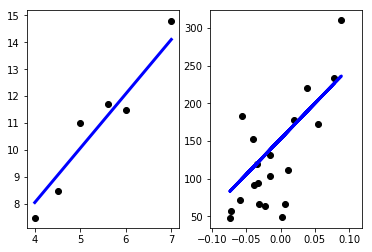
\includegraphics[height=0.3\textheight,width=0.8\linewidth]{r-squared-comparison.png}
	\caption{sample regression fits}
	\label{fig:sample regression fits}
\end{figure}

The r-squared for the regression model on the left is $93\%$ and for the model on the right it is $47\%$. When a regression model accounts for more of the variance, the data points are closer to the regression line. In practice, a regression model with $R^2$ of $100\%$ is never observed. In that case fitted values equal the data values and consequently all observation fall exactly on the regression line.

The below function can be used as a reference to implement r-squared in Rust. We first take the model variance which is the sum of the squares of consecutive difference between actual and predicted values. Then we take the mean of the actual distribution and use that to calculate the variance of the test distribution. Then we run it through the r-squared formula.

\begin{lstlisting}[caption={ml\\-utils\\/src\\/sup\_metrics\\.rs}]
fn r_squared_score(y_test: &Vec<f64>, y_preds: &Vec<f64>) -> f64 {
  let mv: f64 = y_test.iter().zip(y_preds.iter()).fold(
    0., |v, (y_i, y_i_hat)| {
      v + (y_i - y_i_hat).powi(2)
    }
  );

  let mean = y_test.iter().sum::<f64>() as f64
    / y_test.len() as f64;

  let var =  y_test.iter().fold(
    0., |v, &x| {v + (x - mean).powi(2)}
  );
  let r2: f64 = 1.0 - (mv / var);
  r2
}
\end{lstlisting}

This function should not be usable by passing the \lstinline{y_test} and \lstinline{y_pred} to get the score. Since in the examples in this chapter the \lstinline{y_test} and predicted values are in \lstinline{rusty-machine} Matrices we will probably need to do something like below.

\begin{lstlisting}[caption={chapter2\\/rustlymachine\_regression/src\\/glms\\.rs}]
println!("glm poisson R2 score: {:?}", r_squared_score(
    &boston_y_test.data(), &predictions.data()));
\end{lstlisting}
\label{sub:r_squared_error}

\label{sub:evaluation_of_rusty_machine_models}

\section{Classification Algorithms}%

Scenarios where the machine learning algorithm is tasked with bucketing input variables to predefined buckets are called classification problems. In this section we will be creating classification models in Rust.

In Rust we can create classifiers using the package \lstinline{rustlearn}. This crate contains effective implementation for a number of common machine learning algorithms. To be able to use \lstinline{rustlearn}, we will need to implement the floats as \lstinline{float32}.

\subsection{Iris Data Set}%

\paragraph{}%
For showing the usage of the classification algorithms we will be using the iris dataset\footnote{\href{https://archive.ics.uci.edu/ml/datasets/iris}{Iris Data Set}}. It is a multivariate data set with the following features.

\begin{itemize}
	\item Sepal length in cm
	\item sepal width in cm.
	\item petal length in cm.
	\item petal width in cm.
	\item classes: setosa, versicolor and virginica.
\end{itemize}

The code that is explained here is kept in the \lstinline{rustlearn_classification_tasks} folder. Inside the package create a folder \lstinline{data} and keep the csv file there.
\label{par:}

\begin{lstlisting}[language=bash,caption={iris data}]
$ head -n2 data/iris.csv
sepal_length,sepal_width,petal_length,petal_width,species
5.1,3.5,1.4,0.2,setosa
$ wc -l data/iris.csv
151 data/iris.csv # there are 150 samples in the data set.
\end{lstlisting}

Similar to before we are going to work with \lstinline{rustlearn}, \lstinline{csv}, \lstinline{rand} and \lstinline{serde}. Find these dependencies in the \lstinline{Cargo.toml} file.

\begin{lstlisting}[caption={Cargo\\.toml}]
[dependencies]
rustlearn = "0.5.0"
csv = "1.0.5"
serde = "1.0.89"
rand = "0.6"
\end{lstlisting}

\paragraph{}%
Remember that in the regression case we created a \lstinline{BostonHousing} \lstinline{struct}. In this case we are going ahead with creating a \lstinline{Flower} \lstinline{struct}. Notice that the code structures will be largely similar.
\label{par:}

\begin{lstlisting}[caption={ml\\-utils\\/src\\/datasets\\.rs}]
extern crate serde;
#[macro_use]
extern crate serde_derive;

#[derive(Debug, Deserialize)]
struct Flower {
  sepal_length: f32, sepal_width: f32,
  petal_length: f32, petal_width: f32,
  species: String,
}
\end{lstlisting}

Here species is the label and other columns are the features. So to parse out the features and the labels we will implement \lstinline{into_feature_vector} and \lstinline{into_labels} for the \lstinline{Flower} \lstinline{struct}. Note that in case of defining the feature vector the order of the placement in the csv file is maintained. And in case of label encoding some numbers (which are arbitrary) are given to the different labels. Ideally along with a label encoding method a label decoder should also be implemented for the final response. In this case for the sake of brevity that is not shown.

\begin{lstlisting}[caption={ml\\-utils\\/src\\/datasets\\.rs}]
use std::io; use std::vec::Vec; use csv;
impl Flower {
  fn into_feature_vector(&self) -> Vec<f32> {
    vec![self.sepal_length, self.sepal_width,
    self.sepal_length, self.petal_width]
  }

  fn into_labels(&self) -> f32 {
    match self.species.as_str() {
      "setosa" => 0., "versicolor" => 1.,
      "virginica" => 2.,
      some_other => panic!("Not able to parse the label.
        Some other label got passed. {:?}", some_other),
    }
  }
}
\end{lstlisting}

We will use the amazing \lstinline{stdin} and read the package using a command similar to \lstinline{cargo run lr < data/iris.csv}. Here \lstinline{cargo run} will compile and run the binary and \lstinline{lr} is the argument after that which is enabled in the package. Take a look at \lstinline{main.rs} for all the options. So to enable that we will use the \lstinline{std::io} package and pass it to a \lstinline{rdr} variable using \lstinline{csv::Reader}. We now serialize each record to the \lstinline{Flower} \lstinline{struct} and push it to and push it to a data vector, a similar data vector that we h ave seen in the regression section. With this we will also shuffle the data for good measure.

\begin{lstlisting}[caption={chapter3\\/rustlearn\_classification\_tasks\\/src\\/logistic\_reg\\.rs}]
use ml_utils::datasets::Flower;

use csv; use rand::thread_rng;
use rand::seq::SliceRandom;
let mut rdr = csv::Reader::from_reader(io::stdin());
let mut data = Vec::new();
for result in rdr.deserialize() {
  let r: Flower = result?; // should have Box<Error> in the defn.
  data.push(r);
}
data.shuffle(&mut thread_rng());
\end{lstlisting}

Now we will be separating out the train and test datasets. The code is similar to the one in regression section except here in this case we will need to convert the vectors into \lstinline{rustlearn} sparse or dense vectors.

\begin{lstlisting}[caption={chapter3\\/rustlearn\_classification\_tasks\\/src\\/logistic\_reg\\.rs}]
use rustlearn::prelude::*;

// separate out to train and test datasets.
let test_size: f32 = 0.2;
let test_size: f32 = data.len() as f32 * test_size;
let test_size = test_size.round() as usize;
let (test_data, train_data) = data.split_at(test_size);
let train_size = train_data.len();
let test_size = test_data.len();

// differentiate the features and the labels.
let flower_x_train: Vec<f32> = train_data.iter()
  .flat_map(|r| r.into_feature_vector()).collect();
let flower_y_train: Vec<f32> = train_data.iter()
  .map(|r| r.into_labels()).collect();
let flower_x_test: Vec<f32> = test_data.iter()
  .flat_map(|r| r.into_feature_vector()).collect();
let flower_y_test: Vec<f32> = test_data.iter()
  .map(|r| r.into_labels()).collect();

// Convert the vectors to a dense matrix or a sparse matrix
let mut flower_x_train = Array::from(flower_x_train);
flower_x_train.reshape(train_size, 4);
let flower_y_train = Array::from(flower_y_train);
let mut flower_x_test = Array::from(flower_x_test);
flower_x_test.reshape(test_size, 4);
\end{lstlisting}

We should now be able to train the data on \lstinline{rustlearn} models.
\label{sub:iris_data_set}

\subsection{Logistic Regression}%
\paragraph{}%
Logistic Regression is a popular classification technique in which a logit function is used to model a binary dependent variable. The assumption for the dependent variable is that it follows Bernoulli distribution. While OLS regression is a distance-minimizing approximation method, estimation of parameters is done using the maximum likelihood method. Maximizing the likelihood function determines the parameters that are most likely to produce the observed data.
\label{par:}

Unlike regression, for normally distributed residuals, it is not possible to find a closed form solution that maximize the function. So an iterative approach has to be used. One of the popular iterative approaches is Stochastic Gradient Descent. SGD is implemented in \lstinline{rustlearn} and to implement model training in \lstinline{rustlearn} we call the \lstinline{Hyperparameter} module from \lstinline{linear_models} and can pass various parameters such as learning rate, l1 and l2 penalties and if it is a multilabel classification or binary classification.

\begin{lstlisting}[caption={chapter3\\/rustlearn\_classification\_tasks\\/src\\/logistic\_reg\\.rs}]
use rustlearn::linear_models::sgdclassifier::Hyperparameters as lr;
let mut model = lr::new(4)
  .learning_rate(0.1).l2_penalty(0.5)
  .l1_penalty(0.0).one_vs_rest();
for _ in 0..100 { // for 100 epochs
  model.fit(&flower_x_train, &flower_y_train).unwrap();
}
\end{lstlisting}
Running the for loop on the model is equivalent to training the model for multiple epochs.
\label{par:model_training}

\label{sub:logistic_regression}

\subsection{Decision Trees}%
Let us try to redefine the classification problem and understand it from a different perspective. In a classification problem, we have a training sample of $n$ observations on a class variable $Y$ that takes values $1, 2, ..., k$ and $p$ predictor variables, $X_1, X_2, ..., X_p$ Our goal is to find a model for predicting the values of Y for new X values. We can think of this problem as simply a partition of the X-space into $k$ disjoint sets, $A_1, A_2, ..., A_k$, such that the predicted value of Y is j if $X$ belongs to $A_j$, for $j = 1, 2, ..., k$. Classification trees take this approach. They yield rectangular sets $A_j$ by recursively partitioning the data set one $X$ variable at a time. This makes the sets easier to interpret. A key advantage of the tree structure is its applicability to any number of variables.

The key idea is:

\begin{enumerate}
	\item Grow an overly large tree by using forward selection. At each step, find the best split. Grow until all terminal nodes either
		\begin{enumerate}
			\item have $< n$ data points,
			\item all nodes in a node have the same outcome. If this happens the node is said to be "pure".
		\end{enumerate}
	\item Prune the tree back, creating a nested sequence of trees, decreasing in complexity.
\end{enumerate}

where $\chi_m$ is the training data in the node $m$.

Implementing decision trees in \lstinline{rustlearn} can be done with the below code. It supports CART algorithm for both dense and sparse data and features are selected using reduction in Gini impurity\cite{WEBSITE:7}.

\begin{lstlisting}[caption={chapter3\\/rustlearn\_classification\_tasks\\/src\\/trees\\.rs}]
use rustlearn::trees::decision_tree;
let mut tree_params = decision_tree::Hyperparameters::new(
  flower_x_train.cols());
tree_params.min_samples_split(10)
 .max_features(4).min_samples_split(5)
 .max_depth(40).one_vs_rest();
\end{lstlisting}

\label{sub:Decision trees}

\subsection{Random Forest}%
As an improvement of decision trees is the Random Forest. In this case an ensemble of trees is grown and voting is done among them to get the most popular class. The trees are a combination of tree predictors such that each tree depends on the values of a random vector sampled independently and with the same distribution for all trees in the forest. The generalization for the forests converges to a limit as the number of trees in the forest becomes large\cite{WEBSITE:10} .

To implement random forests in \lstinline{rustlearn} we will need to pass the previous decision trees variable with the parameters to the random forest \lstinline{hyperparameter} module so that a collection of trees can be built.

\begin{lstlisting}[caption={chapter3\\/rustlearn\_classification\_tasks\\/src\\/trees\\.rs}]
use rustlearn::ensemble::random_forest::Hyperparameters as rf;
let mut model = rf::new(tree_params, 10)
  .one_vs_rest();
model.fit(&flower_x_train,
          &flower_y_train)?;
\end{lstlisting}
\label{sub:random_forest}

\subsection{XGBoost}%
To get even better at creating a good classification model using trees, one idea is to assemble a series of weak learners to convert them into a strong classifier. XGBoost means Extreme Gradient Boosting, so lets take those terms apart one by one. In boosting the trees are built sequentially so that each subsequent tree aims to reduce the errors of the previous tree. Each tree learns from its predecessors and updates the residual errors. Hence the tree that learns next in the sequence will learn from an updated version of the residuals. This results in really strong classifiers\cite{WEBSITE:12}.

In contrast to Random Forest, where the trees are grown to the maximum extent, boosting makes use of trees with fewer splits. Such small trees, which are not very deep, are highly interpretable. Cross-validation is an important step in boosting as this is used to find optimal parameters such as number of tress or iterations, the rate at which the gradient boosting learns, and the depth of the tree.

\paragraph{Parameters}%
Before running XGBoost, we must set three types of parameters: general parameters, booster parameters and task parameters\cite{Chen:2016:XST:2939672.2939785} .

\paragraph{}%
In this case instead of \lstinline{rustlearn} we will be using the \lstinline{rust-xgboost} library \footnote{\href{https://github.com/davechallis/rust-xgboost}{Rust XGBoost Source}}. The full code is kept in the package \lstinline{iris_classification_xgboost} for reference. This library is a wrapper around the XGBoost library \footnote{\href{https://github.com/dmlc/xgboost/}{Original C++ based XGBoost source}}.

In this case we will need to have \lstinline{xgboost = "0.1.4"} which is a wrapper over \lstinline{XGBoost-v0.82}. In the \lstinline{main.rs} we will call the relevant modules.

\begin{lstlisting}[caption={chapter3\\/iris\_classification\_xgboost\\/src\\/main\\.rs}]
use xgboost;
use xgboost::{parameters, DMatrix, Booster};
\end{lstlisting}

The other data preprocessing steps are the same as we have used in the previous sections for logistic regression for the Iris data set. Once the vectors \lstinline{flower_x_train}, \lstinline{flower_y_train}, \lstinline{flower_x_test}, and \lstinline{flower_y_test} vectors are created we will need to convert it to XGBoost compatible vectors though. The \lstinline{x} vectors are converted to \lstinline{DMatrix} and the corresponding labels are set.

\begin{lstlisting}[caption={chapter3\\/iris\_classification\_xgboost\\/src\\/main\\.rs}]
let mut dtrain = DMatrix::from_dense(&flower_x_train, train_size).unwrap();
dtrain.set_labels(&flower_y_train).unwrap();

let mut dtest = DMatrix::from_dense(&flower_x_test, test_size).unwrap();
dtest.set_labels(&flower_y_test).unwrap();
\end{lstlisting}

Now we will set the XGBoost parameters. First the objective function will be set to Multilabel Softmax as the number of labels are more than 2.  Then we will set the tree based learning model's parameter. These are utilised in setting the booster configuration.

\begin{lstlisting}[caption={chapter3\\/iris\_classification\_xgboost\\/src\\/main\\.rs}]
let lps = parameters::learning::LearningTaskParametersBuilder::default()
  .objective(parameters::learning::Objective::MultiSoftmax(3))
  .build().unwrap();
let tps = parameters::tree::TreeBoosterParametersBuilder::default()
  .max_depth(2).eta(1.0)
  .build().unwrap();
let bst_parms = parameters::BoosterParametersBuilder::default()
  .booster_type(parameters::BoosterType::Tree(tps))
  .learning_params(learning_params)
  .verbose(true).build().unwrap();
\end{lstlisting}

After that we will specify which matrices are for training and which for testing. This will be passed to a configuration object that will be utilised during the training.

\begin{lstlisting}[caption={chapter3\\/iris\_classification\_xgboost\\/src\\/main\\.rs}]
let ev = &[(&dtrain, "train"), (&dtest, "test")];
let params = parameters::TrainingParametersBuilder::default()
  .dtrain(&dtrain).boost_rounds(2)
  .booster_params(bst_parms)
  .evaluation_sets(Some(ev))
  .build().unwrap();
let booster = Booster::train(&params).unwrap();
\end{lstlisting}

Now the predictions can be taken and compared with the actual values.

\begin{lstlisting}[caption={chapter3\\/iris\_classification\_xgboost\\/src\\/main\\.rs}]
let preds = booster.predict(&dtest).unwrap();
let labels = dtest.get_labels().unwrap();

// find the accuracy
let mut hits = 0;
let mut correct_hits = 0;
for (predicted, actual) in preds.iter().zip(labels.iter()) {
  if predicted == actual {
    correct_hits += 1;
  }
  hits += 1;
}
assert_eq!(hits, preds.len());
println!("accuracy={} ({}/{} correct)",
  correct_hits as f32 / hits as f32, correct_hits, preds.len());
\end{lstlisting}

The accuracy should be around 93-96\%.

\label{par:rust_xgboost}

\label{sub:xgboost}

\subsection{Support Vector Machines}%
A Support Vector Machine (SVM) is a discriminative classifier formally defined by a separating hyperplane. In other words given labeled training data, the algorithm outputs an optimal hyperplane which categorizes new examples. In two dimensional space this hyperplane is a line dividing a plane into two parts where in each class lay on either side. The vectors that define the hyperplane are the support vectors.

Kernel functions change the definition of the dot product in the linear formulation. The different types of common dot products are linear, polynomial, radial basis functions and sigmoid functions. Generally RBF functions are taken as the default kernels in most svm models\cite{svm}.

In the Figure 1 with different data points, multiple hyperplanes are experimented with but the hyperplane (line2) is chosen because it has the highest degree of margin.

\begin{figure}
	\centering
	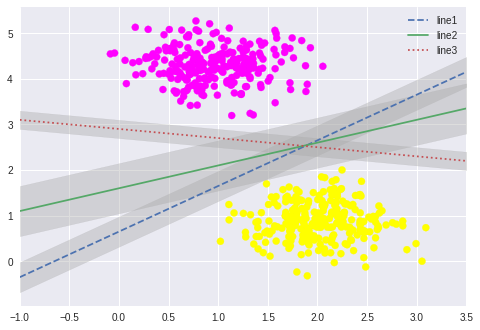
\includegraphics[width=0.8\linewidth]{svm.png}
	\caption{Svm}
	\label{fig:svm}
\end{figure}

To implement SVM in \lstinline{rustlearn} we will need to create the model with the appropriate kernel function first and fit the model on the training data set. The SVM module in \lstinline{rustlearn} is just a wrapper over the \lstinline{libsvm} package\footnote{\href{https://www.csie.ntu.edu.tw/~cjlin/libsvm/}{libsvm}}. Observe the below snippet where the models for the different kernels are shown together.

\begin{lstlisting}[caption={chapter3\\/rustlearn\_classification\_tasks\\/src\\/trees\\.rs}]
use rustlearn::svm::libsvm::svc::{Hyperparameters as libsvm_svc, KernelType};
let svm_linear_model = libsvm_svc::new(
  4, KernelType::Linear, 3)
  .C(0.3).build();
let svm_poly_model = libsvm_svc::new(4, KernelType::Polynomial, 3)
  .C(0.3) .build();
let svm_rbf_model = libsvm_svc::new(4, KernelType::RBF, 3)
  .C(0.3).build();
let svm_sigmoid_model = libsvm_svc::new(4, KernelType::Sigmoid, 3)
  .C(0.3).build();
let svm_kernel_types = ["linear", "polynomial", "rbf", "sigmoid"];
let mut svm_model_types = [svm_linear_model, svm_poly_model, svm_rbf_model, svm_sigmoid_model];
for (kernel_type, svm_model) in svm_kernel_types.iter().zip(svm_model_types.iter_mut()) {
  svm_model.fit(&flower_x_train, &flower_y_train).unwrap();

  let prediction = svm_model.predict(&flower_x_test).unwrap();
  let acc = accuracy_score(&flower_y_test, &prediction);
  println!("Lib svm {kernel}: accuracy: {accuracy}", accuracy=acc, kernel=kernel_type);
};
\end{lstlisting}

We should be getting an output similar to below.

\begin{lstlisting}[caption={output}]
Lib svm linear: accuracy: 0.9
Lib svm polynomial: accuracy: 0.9
Lib svm rbf: accuracy: 0.8666667
Lib svm sigmoid: accuracy: 0.26666668
\end{lstlisting}


\label{sub:support_vector_machines}

\subsection{K Nearest Neighbors}%
For classification in Rust we have mostly been focused on \lstinline{rustlearn} and for regression we have used \lstinline{rusty-machine}, but one of the popular classifiers that is available in rusty-machine and not in \lstinline{rustlearn} is the K nearest neighbors algorithm. The assumption in KNN algorithm is that "birds of the same feather flock together" or similar things tend to have the same results. So an object is classified by the plurality vote of the neighbors.

In rusty-machine, the KNN classifiers have not been published on the crate and hence we will need to clone the repo and build from the path or use the github reference.

\begin{lstlisting}[caption={chapter2\\/rusty\_machine\_classification\\/Cargo\\.toml}]
[dependencies]
rusty-machine = { path = "../rusty-machine" }
ml-utils = { path = "../ml-utils" }
rand = "0.6.5"
csv = "1.0.7"
\end{lstlisting}

Since this is a classification algorithm, we will be using the Flower struct and iris data set. The Flower struct has been implemented for usage with \lstinline{rustlearn} and hence we will need to do some extra maneuvering.

\begin{lstlisting}[caption={chapter2\\/rusty\_machine\_classification\\/Cargo\\.toml}]
use rusty_machine as rm;
use rm::linalg::Matrix;
use rm::linalg::Vector;

use ml_utils;
use ml_utils::datasets::Flower;

// differentiate the features and the labels.
let flower_x_train: Vec<f64> = train_data.iter().flat_map(|r| {
  let features = r.into_feature_vector();
  let features: Vec<f64> = features.iter().map(
    |&x| x as f64).collect();
  features
}).collect();
let flower_y_train: Vec<usize> = train_data.iter().map(
  |r| r.into_int_labels() as usize).collect();

let flower_x_test: Vec<f64> = test_data.iter().flat_map(|r| {
  let features = r.into_feature_vector();
  let features: Vec<f64> = features.iter().map(
    |&x| x as f64).collect();
  features
}).collect();
let flower_y_test: Vec<u32> = test_data.iter().map(
  |r| r.into_int_labels() as u32).collect();

// COnvert the data into matrices for rusty machine
let flower_x_train = Matrix::new(train_size, 4, flower_x_train);
let flower_y_train = Vector::new(flower_y_train);
let flower_x_test = Matrix::new(test_size, 4, flower_x_test);
\end{lstlisting}

Remember that \lstinline{rustlearn} needed vectors of \lstinline{f32}, while in rusty-machine we needed to create \lstinline{rulinalg} matrices of \lstinline{f64}, hence we need to convert these f32 vectors to f64 and then create the matrices in the above code. Also the \lstinline{into_int_labels} of the \lstinline{Flower} struct is the same as \lstinline{into_labels} but implemented for \lstinline{u64} as we are dealing with specific labels in this case.

\begin{lstlisting}[caption={chapter2\\/rust\\-lang\\/ml\\-utils\\/src\\/datasets\\.rs}]
impl Flower {
  // ... previous code for Flower

  pub fn into_int_labels(&self) -> u64 {
    match self.species.as_str() {
      "setosa" => 0,
      "versicolor" => 1,
      "virginica" => 2,
      l => panic!(
        "Not able to parse the target.
	Some other target got passed. {:?}", l),
    }
  }
}
\end{lstlisting}

This was converted to \lstinline{usize} as the KNN \lstinline{struct} that we are going to use later implemented labels as \lstinline{usize}.

We should now be able to create a simple KNN classifier and train it on the iris data set.

\begin{lstlisting}[caption={chapter2\\/rusty\_machine\_classification\\/src\\/main\\.rs}]
use rm::learning::knn::KNNClassifier;
use rusty_machine::learning::knn::{KDTree, BallTree, BruteForce};
use rm::learning::SupModel;
use ml_utils::sup_metrics::accuracy;

let mut knn = KNNClassifier::new(2); // model initialisation
knn.train(&flower_x_train, &flower_y_train).unwrap(); // training

let preds = knn.predict(&flower_x_test).unwrap(); // prediction

let preds: Vec<u32> = preds.data().iter().map(|&x| x as u32).collect();
println!("accuracy {:?}", accuracy(preds.as_slice(), &flower_y_test)); // accuracy
\end{lstlisting}

The accuracy reported should be around $93-100\%$.

In rusty-machine we can have different KNN models apart from the default one which is the KDTree algorithm. We can use the Ball tree algorithm, which is used when the number of dimensions are huge, or the Brute force algorithm, the advantage of which is that it is embarrassingly parallelizable.

\begin{lstlisting}[caption={chapter2\\/rusty\_machine\_classification\\/src\\/main\\.rs}]
use rusty_machine::learning::knn::{KDTree, BallTree, BruteForce};

let mut knn = KNNClassifier::new_specified(2, BallTree::new(30));

let mut knn = KNNClassifier::new_specified(2, KDTree::default());

let mut knn = KNNClassifier::new_specified(2, BruteForce::default());
\end{lstlisting}

For the whole code take a look at the \lstinline{rusty_machine_classification} package in chapter2 folder.
\label{sub:k_nearest_neighbors}

\subsection{Neural Networks}%

Neural networks are a set of algorithms, modeled loosely after the human brain, that are designed to recognize patterns. One of the most popular ways of using neural networks is by grouping them in stacks. Usable networks that work are seen to be composed of several layers. The layers are made of nodes. A node is just a place where computation happens. A node combines input from the data with a set of coefficients or weights, that either amplify or dampen that input, thereby assigning significance to inputs with regard to the task the algorithm is trying to learn, for example which input is most helpful in classifying the data without error. These input weight products are summed and passed through an "activation function". Activation functions are generally non-linear and they work to determine whether and to what extent that signal should progress further through the network to affect the ultimate outcome, an example being the classification task. If the signal passes through, the neuron has been "activated". Take a look at Figure 2 to have an understanding of how a node might look like.

\begin{figure}
	\centering
	\includegraphics[width=0.8\linewidth]{single_node.png}
	\caption{single node example}
	\label{fig:single node example}
\end{figure}

A node layer is a row of those neuron like switches that turn on and off as the input is fed through the net. Each layers output is simultaneously the next layers input, starting from an initial input layer receiving the data. Pairing the models adjustable weights with input features is how we assign significance to those features with regard to how the neural network classifies and clusters input.

\begin{figure}
	\centering
	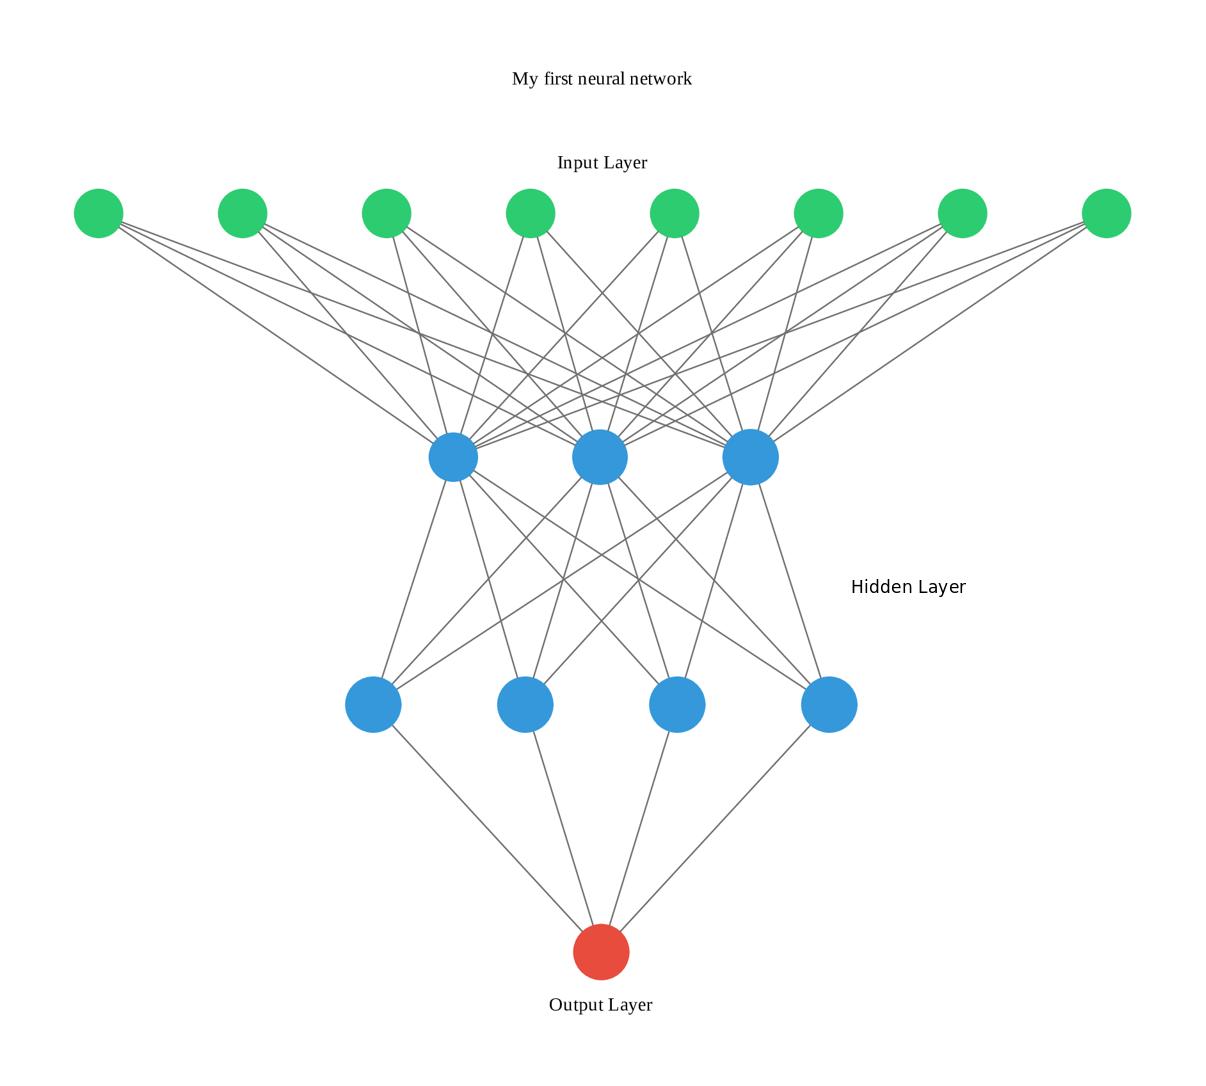
\includegraphics[width=0.8\linewidth]{deep_neural_network.png}
	\caption{deep neural network}
	\label{fig:deep neural network}
\end{figure}

Neural networks with multiple hidden layers have each layer of node train on a distinct set of features based on the previous layer's output. More deep layers learn the more complicated features in the training data, since they are able to aggregate and recombine features from the previous layers.

\paragraph{}%
\textbf{Torch and tch-rs}

Torch is a scientific computing framework with wide support for machine learning algorithms and has good support for GPU\cite{WEBSITE:15} . It is hence widely used for deep learning and creating neural network architectures. The C implementation of Torch is distributed in a package called \lstinline{libtorch}. It provides a flexible N-dimensional array or tensor, which supports basic routines for indexing. slicing, transposing, type-casting, resizing, sharing storage and cloning. This object is used by most other packages and useful and more complicated routines are built on top of it.

In Rust, the \lstinline{libtorch} C++-api has been extended using the tch-rs crate \footnote{\href{https://github.com/LaurentMazare/tch-rs}{tch-rs}}. The aim of this create is to be as close to the C++ api as possible.

To use \lstinline{tch-rs} just adding \lstinline{tch-rs} in your \lstinline{Cargo.toml} and then doing a \lstinline{cargo build} should work. In case you are in a Mac system and encounter the below error

\begin{lstlisting}[caption={}]
dyld: Library not loaded: @rpath/libmklml.dylib
  Referenced from: /path to libtorch/lib/libcaffe2.dylib
  Reason: image not found
\end{lstlisting}

We can resolve this error by manually downloading the file and adding the paths to the lib file in the mac terminal


\begin{lstlisting}[caption={installation}]
$ wget https://github.com/intel/mkl-dnn/releases/download/v0.18/mklml_mac_2019.0.3.20190220.tgz
$ gunzip -c mklml_mac_2019.0.3.20190220.tgz| tar xvf -
$ export LD_LIBRARY_PATH=/path to mkl folder/lib:"$LD_LIBRARY_PATH"
\end{lstlisting}

The code should build after this.

We will now build a small neural network on it so that the network can train on the data. To be able to do that we will need to change the data though. We will take a look at all the important steps next. These steps are under the assumption that all the data preprocessing steps are complete and are similar to the ones we encountered in the previous sections. The consolidated code is also present in the package \lstinline{iris_classification_tchrs} for reference.

First we will need to specify the test train ratio to be the same. This is a technicality that needs to be taken care because of the way matrix multiplication works and the implications we will take a look at later. So

\begin{lstlisting}[caption={iris\_classification\_tchrs}]
let test_size: f64 = 0.5;
\end{lstlisting}

Now we will need to convert the vectors to torch Tensors so that we are able to perform computations on those Tensors.

\begin{lstlisting}[caption={chapter3\\/iris\_classification\_tchrs\\/src\\/main\\.rs}]
use tch::{kind, Kind, Tensor};
let flower_x_train = Tensor::float_vec(flower_x_train.as_slice());
let flower_y_train = Tensor::float_vec(flower_y_train.as_slice()).to_kind(Kind::Int64);
let flower_x_test = Tensor::float_vec(flower_x_test.as_slice());
let flower_y_test = Tensor::float_vec(flower_y_test.as_slice()).to_kind(Kind::Int64);
\end{lstlisting}

We can now reshape the vectors to reflect the training size and the dimension of the features. Label values in this case are essentially vectors.

\begin{lstlisting}[caption={chapter3\\/iris\_classification\_tchrs\\/src\\/main\\.rs}]
let train_size = train_size as i64;
let test_size = test_size as i64;
let flower_x_train = flower_x_train.view(&[train_size, 4]);
let flower_x_test = flower_x_test.view(&[test_size, 4]);
let flower_y_train = flower_y_train.view(&[train_size]);
let flower_y_test = flower_y_test.view(&[test_size]);
\end{lstlisting}

Now we come to the actual neural network creation. Similar to figure 2 lets create a single layer network where there such that we are optimizing on the matrix equation $Y = X * W + B$ where all the values are vectors or matrices\cite{WEBSITE:17} . We will need to initiate our weights and biases for this.

\begin{lstlisting}[caption={chapter3\\/iris\_classification\_tchrs\\/src\\/main\\.rs}]
let mut ws = Tensor::ones(
  &[feature_length, 1], kind::FLOAT_CPU)
  .set_requires_grad(true);
let mut bs = Tensor::ones(
  &[train_size], kind::FLOAT_CPU)
  .set_requires_grad(true);
\end{lstlisting}

In the above example we will be setting the \lstinline{requires_grad} to be \lstinline{true} because we will need to compute the gradients for these values. Tensors have \lstinline{requires_grad} as \lstinline{false} by default and gradient for tensors for which the \lstinline{requires_grad} is false are not calculated\cite{WEBSITE:15} .

Now we will need to first perform the matrix multiplication \lstinline{flower_x_train * ws + bs}. We will then consider the loss against \lstinline{flower_y_train}. We will now need to propagate the loss. This operation will be repeated for multiple epochs and we will report the accuracy for each epoch so that we are able to keep track of increase or decrease in accuracy of the model.

\begin{lstlisting}[caption={chapter3\\/iris\_classification\_tchrs\\/src\\/main\\.rs}]
for epoch in 1..200 {
  let logits = flower_x_train.mm(&ws) + &bs;
  let loss = logits.squeeze().cross_entropy_for_logits(&flower_y_train);
  ws.zero_grad();
  bs.zero_grad();
  loss.backward();
  no_grad(|| {
    ws += ws.grad() * (-1);
    bs += bs.grad() * (-1);
  });
  let test_logits = flower_x_test.mm(&ws) + &bs;
  let test_accuracy = test_logits
    .argmax1(-1, false)
    .eq1(&flower_y_test)
    .to_kind(Kind::Float)
    .mean()
    .double_value(&[]);
  println!(
    "epoch: {:4} train loss: {:8.5} test acc: {:5.2}%",
    epoch,
    loss.double_value(&[]),
    100. * test_accuracy
  );
}
\end{lstlisting}

Running this model we should see incremental decrease in the loss of the model.
\label{par:}
\paragraph{Linear network using Torch}%
Now creating the previous model is great for understanding of neural networks but there is a better way of creating networks in torch similar to what is advocated for in \lstinline{pytorch} as well. For creating models in torch we can create a simple \lstinline{struct} and then implement forward for the struct.

\begin{lstlisting}[caption={chapter2\\/iris\_classification\_tchrs\\/src\\/linear\_with\_sgd\\.rs}]
use tch;
use tch::{nn, kind, Kind, Tensor, no_grad, vision, Device};
use tch::{nn::Module, nn::OptimizerConfig};

static FEATURE_DIM: i64 = 4;
static HIDDEN_NODES: i64 = 10;
static LABELS: i64 = 3;

#[derive(Debug)]
struct Net {
  fc1: nn::Linear,
  fc2: nn::Linear,
}

impl Net {
  fn new(vs: &nn::Path) -> Net {
    let fc1 = nn::Linear::new(vs,
      FEATURE_DIM, HIDDEN_NODES,
      Default::default());
    let fc2 = nn::Linear::new(vs,
      HIDDEN_NODES, LABELS,
      Default::default());
    Net { fc1, fc2 }
  }
}

impl Module for Net {
  fn forward(&self, xs: &Tensor) -> Tensor {
    xs.apply(&self.fc1).relu().apply(&self.fc2)
  }
}
\end{lstlisting}

In the above model we create two linear networks, basically a hidden network between the input layer and the output labels. The \lstinline{forward} method is then overriden to implement the network.

To train the above network we will need to convert the \lstinline{Flower} vectors to torch tensors.

\begin{lstlisting}[caption={}]
let flower_x_train = Tensor::float_vec(
  flower_x_train.as_slice());
let flower_y_train = Tensor::float_vec(
  flower_y_train.as_slice()).to_kind(Kind::Int64);
let flower_x_test = Tensor::float_vec(
  flower_x_test.as_slice());
let flower_y_test = Tensor::float_vec(
  flower_y_test.as_slice()).to_kind(Kind::Int64);

let train_size = train_size as i64;
let test_size = test_size as i64;
let flower_x_train = flower_x_train.view(&[train_size, FEATURE_DIM]);
let flower_x_test = flower_x_test.view(&[test_size, FEATURE_DIM]);
let flower_y_train = flower_y_train.view(&[train_size]);
let flower_y_test = flower_y_test.view(&[test_size]);
\end{lstlisting}

Now that the model and the appropriate tensors have been created we should be able to train the model using stochastic gradient descent algorithm.

\begin{lstlisting}[caption={}]
let vs = nn::VarStore::new(Device::Cpu); // use GPU for bigger models.
let net = Net::new(&vs.root());
let opt = nn::Adam::default().build(&vs, 1e-3)?;
for epoch in 1..200 {
  let loss = net
    .forward(&flower_x_train)
    .cross_entropy_for_logits(&flower_y_train);
  opt.backward_step(&loss);
  let test_accuracy = net
    .forward(&flower_x_test)
    .accuracy_for_logits(&flower_y_test);
  println!(
    "epoch: {:4} train loss: {:8.5} test acc: {:5.2}%",
    epoch,
    f64::from(&loss),
    100. * f64::from(&test_accuracy),
  );
};
\end{lstlisting}

We should be able to run the command \lstinline{cargo run linear_with_sgd < data/iris.csv} to run this linear model.

\label{par:linear_network_using_torch}

\label{sub:neural_networks}

\subsection{Model Evaluation}%

\paragraph{Accuracy}%
The most common metric to evaluate a classification model is by using classification accuracy. It is the ratio of the number of correct predictions to the total number of input samples.

\begin{equation}
	\text{Accuracy} = \frac{\text{Number of correct predictions}}{\text{Total number of predictions made}}
\end{equation}

We can implement this using the below function

\begin{lstlisting}[caption={ml\\-utils\\/src\\/sup\_metrics\\.rs}]
pub fn accuracy(y_test: &[u32], y_preds: &[u32]) -> f32 {
  let mut correct_hits = 0;
  for (predicted, actual) in y_preds.iter().zip(y_test.iter()) {
    if predicted == actual {
      correct_hits += 1;
    }
  }
  let acc: f32 = correct_hits as f32 / y_test.len() as f32;
  acc
}
\end{lstlisting}

The signature of the function is \lstinline{u32} because the y values will be specific labels.

Or since we are using \lstinline{rustlearn} in this chapter we can use the \lstinline{accuracy_score} from the package.

\begin{lstlisting}[caption={chapter3\\/rustlearn\_classification\_tasks\\/src\\/logistic\_reg\\.rs}]
use rustlearn::metrics::accuracy_score;

let prediction = model.predict(&flower_x_test).unwrap();
let acc = accuracy_score(&flower_y_test, &prediction);
\end{lstlisting}

Using the above function we should be able to see the following accuracy scores for the models implemented.

\begin{lstlisting}[caption={chapter3\\/rustlearn\_classification\_tasks\\/src\\/logistic\_reg\\.rs}]
$ cargo run lr < data/iris.csv
    Finished dev [unoptimized + debuginfo] target(s) in 3.66s
     Running `target/debug/rustlearn_classification_tasks lr`
Logistic Regression: accuracy: 0.3
Logistic Regression: accuracy: 0.3
\end{lstlisting}

This method of calculating the accuracy score only works if there are equal number of samples belonging to each class. For example lets assume that $99\%$ samples belong to class A and the remaining $1\%$ belong to class B. Then by the above metric a simple model, such as below, that predicts all out of sample classes as class A would have an accuracy of $99\%$.

\begin{lstlisting}[caption={my awesome machine learning model}]
fn model(y_test: &Vec<f32>) -> Vec<String> {
  vec![String::from("Class A"); y_test.len()]
}
\end{lstlisting}

The result would be that we would have a false sense of achieving high accuracy.
\label{par:accuracy}

\paragraph{Logarithmic Loss}%
Logarithmic loss or cross entropy loss, works by penalizing the false classifications. It works well for multi-class classifications. Log Loss increases as the predicted probability diverges from the actual label. An perfect model would have a log loss of 0. So predicting a probability of 0.12 when the actual observation label is 1 would be bad and result in high log loss\cite{WEBSITE:18} . This is given by

\begin{equation}
	H_p(q) = - \frac{1}{N}\sum_{i=1}^{N}y_i \cdot \log(p(y_i)) + (1-y_i) \dot \log(1-p(y_i))
\end{equation}

The graph below shows the range of possible log loss given a true observation of $1$. Log loss is not very steep when the probability is approaching 1 but increases rapidly when the probability is going towards 0. We want the behaviour to be penalized for any errors, but notice how the penalizing is infinite when the predictors are confident and wrong.

\begin{figure}[htpb]
	\centering
	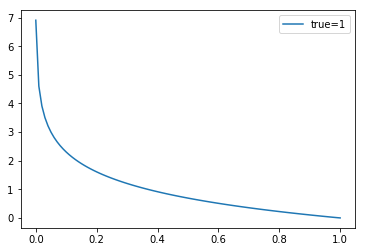
\includegraphics[width=0.8\linewidth]{logloss.png}
	\caption{logloss}
	\label{fig:logloss}
\end{figure}

Thus log loss has a more nuanced approach to accuracy than a simple yes no nature. It gives a value based on how wrong the model is from the true value.

In Rust the below function will calculate the log-loss score. The vectors \lstinline{y_test} and \lstinline{y_preds} are the ground truths and the predicted values. Log-loss is undefined for probability values of 0 and 1 and hence the \lstinline{y_test} vector is clamped to a little above 0 and a little below 1 given by \lstinline{eps} following the equation $\max(\min(p, 1 - \epsilon), \epsilon)$. Note that \lstinline{partial_cmp} is used to compare as we are comparing between two floats. Rust official stance is that comparing floating point numbers is very tricky and situation dependent, and best avoided if at all possible. There is no panacea that "just works"\cite{WEBSITE:19} .

Once done we will implement the actual log-loss function for binary classification on the clamped vector.

\begin{lstlisting}[caption={ml\\-utils\\/src\\/sup\_metrics\\.rs}]
fn logloss_score(y_test: &Vec<f32>,
                 y_preds: &Vec<f32>,
		 eps: f32) -> f32 {
  let y_preds = y_preds.iter().map(|&p| {
    match p.partial_cmp(&(1.0 - eps)) {
      Some(Ordering::Less) => p,
      _ => 1.0 - eps, // if equal or greater.
    }
  });
  let y_preds = y_preds.map(|p| {
    match p.partial_cmp(&eps) {
        Some(Ordering::Less) => eps,
        _ => p,
    }
  });

  let logloss_vals = y_preds.zip(y_test.iter())
    .map(|(predicted, &actual)| {
      if actual as f32 == 1.0 {
        (-1.0) * predicted.ln()
      } else if actual as f32 == 0.0 {
        (-1.0) * (1.0 - predicted).ln()
      } else {
        panic!("Not supported. y_preds should be either 0 or 1");
      }
    });
  logloss_vals.sum()
}
\end{lstlisting}

This can now be used in something similar to below.

\begin{lstlisting}[caption={}]
let preds = vec![1., 0.0001, 0.908047338626,
  0.0199900075962, 0.904058545833, 0.321508119045,
  0.657086320195];
let actuals = vec![1., 0., 0., 1., 1., 0., 0.];
println!("{:?}",
  logloss_score(&actuals, &preds, 1e-15)); // output 7.8581247
\end{lstlisting}
\label{par:logarithmic_loss}

% TODO: implement confusion matrix
%\paragraph{Confusion Matrix}%
%Confusion matrix is a table with rows and columns that report the number of false positives, false negatives, true positives, and true negatives. This allows for a more detailed analysis than the mere proportions of correct classifications. An example of a confusion matrix is sown below.
%
%\begin{center}
%\begin{tabular}{ |c|c|c|c| }
%\hline
%actual/predicted & negative & positive \\
%\hline
%Negative & a & b \\
%Positive & c & d \\
%\hline
%\end{tabular}
%\end{center}
%
%Confusion matrix is implemented in
%
%\label{par:confusion_matrix_}

\paragraph{ROC-AUC}%
An ROC curve(receiver operating characteristic curve) is a graph showing the performance of a classification model at all classification thresholds\cite{WEBSITE:20}. The curve plots two parameters.

\begin{itemize}
	\item True Positive Rate
	\item False Positive Rate
\end{itemize}

True Positive Rate(TPR) is a synonymn for recall and is therefore defined as

\begin{equation}
	\text{TPR} = \frac{\text{TP}}{\text{TP + FN}}
\end{equation}

and False Positive Rate is defined as

\begin{equation}
	\text{FPR} = \frac{FP}{\text{FP + TN}}
\end{equation}

An ROC curve  plots TPR vs FPR at different classification thresholds. Lowering the classification threshold classifies more items as positive, thus increasing both false positives and true positives.

\begin{figure}[htpb]
	\centering
	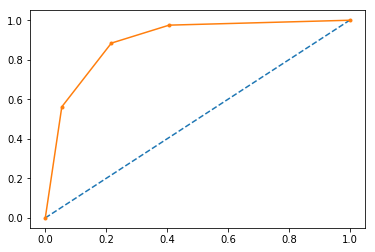
\includegraphics[width=0.8\linewidth]{rocauc.png}
	\caption{roc-auc curve}
	\label{fig:rocauc}
\end{figure}

AUC stands for "Area under the ROC Curve". It measures the entire two dimensional area under the entire ROC Curve. For the figure 5 the ROC-AUC area is 0.895. As evident the score has a range between 0 and 1. The greater the value, the better is the performance of the model.

The crate \lstinline{rustlearn} has roc-auc score implemented for binary classification.

\begin{lstlisting}[caption={chaper3\\/rustlearn\_classification\_tasks\\/src\\/binary\_class\_scores\\.rs}]
use rustlearn::metrics::roc_auc_score;
let preds = vec![1., 0.0001, 0.908047338626, 0.0199900075962,
  0.904058545833, 0.321508119045, 0.657086320195];
let actuals = vec![1., 0., 0., 1., 1., 0., 0.];
println!("roc auc scores: {:?}",
  roc_auc_score(&Array::from(actuals), &Array::from(preds))?); // output: 0.6666667
\end{lstlisting}

Running the above should give something like below.

\begin{lstlisting}[caption={chaper3\\/rustlearn\_classification\_tasks\\/src\\/binary\_class\_scores\\.rs}]
$ cargo run bs
    Finished dev [unoptimized + debuginfo] target(s) in 0.16s
     Running `target/debug/rustlearn_classification_tasks bs`
logloss score: 7.8581247
roc auc scores: 0.6666667
\end{lstlisting}
\label{par:roc_auc}

%% % https://towardsdatascience.com/metrics-to-evaluate-your-machine-learning-algorithm-f10ba6e38234
%% % https://machinelearningmastery.com/how-to-score-probability-predictions-in-python/
%% % https://medium.com/datadriveninvestor/how-to-evaluate-the-performance-of-a-machine-learning-model-45063a7a38a7
%% % https://towardsdatascience.com/metrics-to-evaluate-your-machine-learning-algorithm-f10ba6e38234
%% % https://www.analyticsvidhya.com/blog/2016/02/7-important-model-evaluation-error-metrics/
%
%
%
%\label{sub:model_evaluation}

\label{sec:classification}

\section{Conclusion}
This chapter introduced you to different regression algorithms such as Linear Regression, Gaussian Processes and Generalized Linear Models. Along with the algorithms, the package \lstinline{rusty_machine}  is introduced and how to create regression models of these algorithms using the package. Finally we end the chapter with an understanding of how to evaluate regression models.

In the next chapter you will learn about creating classification models.

\printbibliography
\end{document}
